\chapter{Integrali}

\section{{Integrali a più variabili}}

\subsection{Misura di Peano-Jordan e integrabilità secondo Riemann}

per le funzioni in $\R$ si è definita l'\textbf{integrazione secondo Riemann}, dove bastava che $f(x)$ fosse limitata in un intervallo $[a,b]$ per avere
\begin{align}
	\int_{a}^{b} dx \, f(x)
\end{align}

Riemann può essere esteso ad $\R^2$ tramite la \textbf{misura di Peano-Jordan}. A noi però non interessano, in quanto sono strumenti limitati, come dimostrò Dirichlet con la funzione
\begin{align}
	f(x)=\double{1 \quad x\in [0,1]\cap\Q\quad \;}{0 \quad x\in [0,1], x\notin\Q}
\end{align}
Che non è integrabile in alcun modo con le precedenti definizioni.

Inoltre ci troviamo con le mani legate su molte cose, come lo scambio tra limite e integrale, etc. etc.
Entra quindi in gioco la misura di Lebesgue.

\subsection{Misura di Lebesgue}

\subsubsection{Insiemi misurabili}

La prima domanda che dobbiamo porci è: cos'è un insieme misurabile?

Affrontiamo per semplicità il discorso in $\R^2$, ma le nozioni che verrano date sono estensibili a $\R^n$.

Sia il rettangolo 
\begin{align}
	R= [a_1,b_1]\times [a_2,b_2]
\end{align}

Come sappiamo dalla geometria, una misura sensata della sua area deve dare per forza
\begin{align}
	m(R)=(b_2 - a_2)\cdot(b_1-a_1)
\end{align}

Definiamo ora un \textbf{Plurirettangolo} come l'unione di $n$ rettangoli $R_i$ 
\begin{align}
	P=R_1\cup ... \cup R_n
\end{align}
la cui misura sarà 
\begin{align}
	m(P)= \sum_{i=1}^{n} m(R_i)
\end{align}

Possiamo ora iniziare a studiare domini di forme diverse, usando i Plurirettangoli.

Per esempio dato un insieme aperto $A\neq \emptyset$ possiamo definirne la misura come
\begin{align}
	m(A)=\sup\{ m(P), P\subset A \}
\end{align}

Dato invece un insieme  chiuso $K\neq \emptyset$ possiamo definirne la misura come
\begin{align}
	m(K)=\inf\{ m(P), K\subset P \}
\end{align}

\begin{figure}[!htb]
	\center{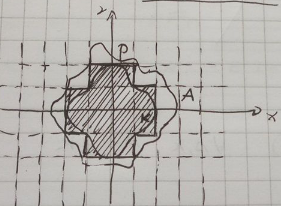
\includegraphics[width=0.5\textwidth]
		{images/insmis.png}
		\caption{Misura in $R^2$}}
\end{figure}

Il caso in $\R^n$ si ottiene generalizzando le formule nel seguente modo:
\begin{align}
	{}&R=[a_1,b_1]\times \dots \times [a_n,b_n]\\
	&m(R)=\prod_{j=1}^{n}(b_j-a_j)\\
	&P= R_1 \cup \dots \cup R_m \spacer R_i \cap R_j = \emptyset \quad \forall i \neq j\\
	&m(P)=\sum_{i=1}^{m}m(R_i)
\end{align}

E le definizioni date per $m(A)$ e $m(K)$ sono identiche a quelle già date.

\newpage

Preso ora un insieme $E \subset \R^n$ possiamo definirne:
\begin{enumerate}
	\item \textbf{Misura esterna:}
	\begin{align}
		\overline{m}(E) = \inf\{m(A), E\subset\underset{aperto}{A}\}
	\end{align} 
	\item \textbf{Misura interna:}
	\begin{align}
		\underline{m}(E) = \sup\{m(K), \underset{chiuso}{K}\subset E\}
	\end{align} 
\end{enumerate}

E affermiamo che $\underline{m}(E) \leq \overline{m}(E)$, dando solo un'idea di dimostrazione:

\bigskip

Se $K \subset E \subset A$ allora $\exists P \taleche K \subset P \subset A$

\bigskip

Questo implica che 
\begin{align}
	m(K)\leq m(P) \leq m(A) \implies m(K)\leq m(A) \quad \forall A,K \taleche K \subset P \subset A
\end{align}

\bigskip

Notiamo ora come preso un dominio aperto $A$ si ha che 
\begin{align}
	{}&m(A)=\overline{m}(A)\\
	&\underline{m}(A)\geq m(P) \quad \forall P \subset A
\end{align}

Ma la seconda equazione ci porta ad avere
\begin{align}
	\underline{m}(A) \geq \sup \{ m(P) \spacecomma \forall P \subset A \} = m(A) \implies \underline{m}(A)\geq m(A)=\overline{m}(A)
\end{align}

Ma per definizione $\overline{m}(A)\geq \underline{m}(A)$ e quindi si ha che
\begin{align}
	\underline{m}(A) =\overline{m}(A) = m(A)
\end{align}

Questo vale non solo per tutti gli aperti $A$, ma anche per i compatti $K$ con procedimento analogo. 

Questo risultato ci tornerà utile nel prossimo paragrafo.

\newpage

\subsubsection{Insiemi misurabili secondo Lebesgue}

Un insieme $E \subset R^n$ si dice misurabile secondo Lebesgue ($L_{mis}$) se
\begin{align}
	{}&\underline{m}(E) =\overline{m}(E) = M  \spacer M= \text{quantità finita}\\
	&m(E)=M
\end{align}

Prendendo in considerazione quanto detto nel paragrafo precente possiamo dire che tutti gli aperti e i compatti sono sempre $L_{mis}$.

Gli insiemi $L_{mis}$ godono delle seguenti proprietà:
\begin{enumerate}
	\item Dati due insiemi $E$ ed $F$ misurabili lo saranno anche 
	\begin{enumerate}
		\item $E\cup F$
		\item $E\cap F$
		\item $E \backslash F$ 
	\end{enumerate}
	\item Sommando i due insiemi si ha $m(E+F)\leq m(E) + m(F)$ e se $E\cap F = \emptyset$ allora $m(E+F)= m(E) + m(F)$
	\item Sommando $n$ domini $E_i$ $L_{mis}$ si ha
	\begin{enumerate}
		\item $	m(E) \leq \sum_{i=1}^{n} m(E_i)$ e si parla di subadditività finita
		\item $m(E) = \sum_{i=1}^{n} m(E_i)$ se $E_i  \cap E_j = \emptyset \quad \forall i,j$ e si parla di additività finita
	\end{enumerate}
\end{enumerate}

\textbf{Nota:} L'insieme degli insiemi misurabili secondo PJ ($PJ_{mis}$) è un sottoinsieme dei $L_{mis}$, in quanto la famiglia di domini integrabili è più restrittiva e si ha
\begin{align}
	{}&\overline{m}_{PJ}(E)=\inf \{ m(\dot{P}), E \subset \dot{P} \} \spacer \dot{P} = \text{plurirett. con punti interni}  \\
	&\underline{m}_{PJ}(E)=\sup \{ m(\dot{P}), \dot{P} \subset E \}
\end{align}

Da cui si ha
\begin{align}
	m\underline{m}_{PJ}(E) \leq \underline{m}_{L}(E) \leq \overline{m}_{L}(E) \leq \overline{m}_{PJ}(E)
\end{align}

E quindi se un insieme è $PJ_{mis}$ è anche $L_mis$.

\begin{figure}[!htb]
	\center{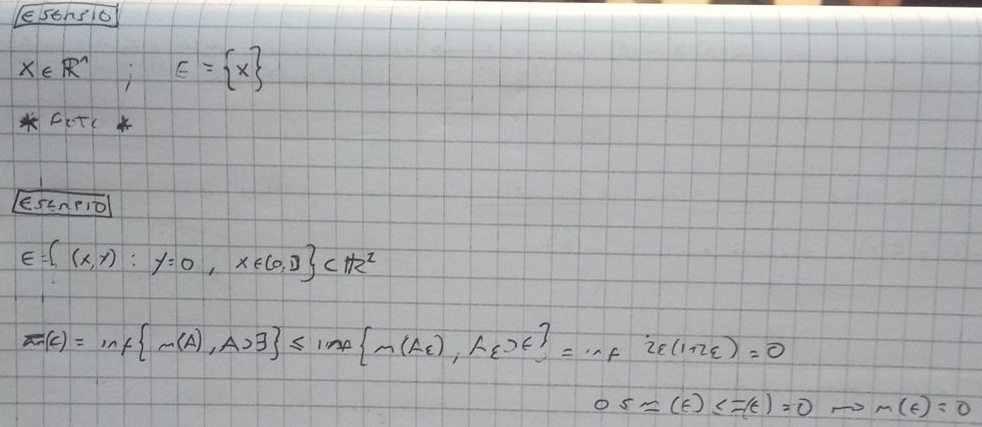
\includegraphics[width=0.8\textwidth]
		{images/insmises.png}
		\caption{\label{fig:my-label}}}
\end{figure}

\newpage

\subsubsection{Teoremi sugli insiemi misurabili}

Diamo ora alcuni teoremi utili ai fini dello studio degli insiemi misurabli.

\begin{enumerate}
	\item \textbf{Teorema dell'additività numerabile della misura}
	
	\textit{Siano $E_1, \dots , E_n$ misurabili, con $E_i \cap E_j =\emptyset \quad \forall i,j$}
	
	\textit{Dato $E= \bigcup_{i=1}^{n} E_i$ se si ha che $\overline{m}(E)< +\infty$ allora}
	
	\textit{E è misurabile e si ha che $m(E)= \sum_{i=1}^{n} m(E_i)$}
	
	\item \textbf{Teorema della subadditività numerabile della misura}
	
	\textit{Siano $E_1, \dots , E_n$ misurabili}
	
	\textit{Dato $E= \bigcup_{i=1}^{n} E_i$ se si ha che $\overline{m}(E)< +\infty$ allora}
	
	\textit{E è misurabile e si ha che $m(E)\leq \sum_{i=1}^{n} m(E_i)$}
	
	\item \textbf{Teorema degli intervalli incapsulati}
	
	\textit{Siano $E_1, \dots , E_n$ misurabili, con $E_1 \subset E_2 \subset \dots \subset E_n$}
	
	\textit{Allora si ha $m(E)= \limit{i}{\infty} m(E_j)$}
\end{enumerate}

\subsubsection{Misurabilità di $\Q\cap [0,1]$ secondo Lebesgue}

Visto che secondo Lebesgue una retta ($ \{ r_j \}$) è un insieme a misura nulla, e dato che
\begin{align}
	\Q \cap [0,1] = \{ r_1, \dots, r_n \} \cdot \{ r_j \}
\end{align}

Si ha che è un insieme a misura nulla.

\subsubsection{Insieme di Cantor}

L'insieme di Cantor viene costruito per ricorrenza nel seguente modo
\begin{align}
	{}&C_0 = [0,1]\\
	&C_1 = C_0 \backslash E_1 \spacer E_1= \left( \frac{1}{3} \spacecomma \frac{2}{3} \right)\\
	&C_2 = C_1 \backslash E_2 \spacer E_2 = \left( \fracn{9} \spacecomma \frac{2}{9} \right) \cup \left( \frac{4}{9} \spacecomma \frac{8}{9} \right)\\
	\vdots
\end{align}

Con
\begin{align}
	\dots \subset C_k \subset C_{k-1}\subset \dots \subset C_0
\end{align}
Da cui si ottiene
\begin{align}
	C= \bigcap_{k=1}^{\infty} C_k = [0,1] \backslash \bigcup_{k=1}^{\infty} E_k
\end{align}

L'insieme di Cantor gode delle seguenti proprietà:
\begin{enumerate}
	\item È un insieme chiuso
	\item $C \neq \emptyset$
	\item non contiene int. (CHE CAZZO VUOL DIRE, CHIEDERE)
	\item Non è numerabile
	\item È misurabile nel seguente modo (si dimostra per induzione)
	\begin{align}
		m(C)= 1 - \sum_{k=1}^{\infty} m(E_k) \spacer m(E_k)= \frac{2^{k-1}}{3^k}
	\end{align} 
\end{enumerate}

\subsubsection{Misurabilità di insiemi chiusi e aperti secondo Lebesgue}

Dato un insieme aperto $E\subset \R^n$, avremo che sarà \Lmis se è misurabile $E\cap B(0,r)$ per ogni $r>0$ e si definisce
\begin{align}
	m(E)= \limit{r}{\infty} m(E\cap B(0,r))
\end{align}

Questo ci permette di poter scrivere
\begin{align}
	\double{\R^n \text{ aperto e misurabile}}{A\subset \R^n \text{ aperto e misurabile}} \implies C= \R^n \backslash A \text{ chiuso e misurabile} \nonumber
\end{align}

\subsubsection{Misura di un prodotto tra spazi}
Dati due spazi $E\subset \R^n$ ed $F\subset \R^k$ a misure rispettivamente $m_n$ ed $m_k$ si ha che dato
\begin{align}
	E \times F = \{ (\vecx,\vecy) , \vecx \in E, \vecy \in F  \}\subset \R^{n+k} \implies m_{n+k}(E\times F) = m_n(E)\times m_k(F)
\end{align}

\section{Integrali di Lebesgue}

Iniziamo il discorso sugli integrali di Lebesgue introducendo le \textbf{funzioni caratteristiche}. Dato un insieme $E\subset \R^n$ avremo
\begin{align}
	\chi_E(\vecx)= \double{1 \quad \vecx\in E}{0 \quad \vecx \notin E}
\end{align}

Avremo che
\begin{align}
	\int_{\R^n} d\vecx \; \chi_E(\vecx)= \int_{\R^n \backslash E} d\vecx \cdot 0 + \int_{E} d\vecx  = m(E)
\end{align}

E possiamo ora definire le \textbf{funzioni semplici} come combinazione lineare di un numero finito di funzioni caratteristiche
\begin{align}
	\Phi(\vecx) = \sum_{j=1}^{n} a_j \chi_{E_j}(\vecx)
\end{align}

Da cui
\begin{align}
	\int_{\R^n} d\vecx  \;  \Phi(\vecx)= \sum_{j=1}^{n} a_j \int_{\R^n} d\vecx  \; \chi_{E_j}(\vecx)=  \sum_{j=1}^{n} a_j m(E_j)
\end{align}

E, prese due funzioni semplici $\Phi$ e $\Psi$ avremo
\begin{enumerate}
	\item \textbf{Linearità:}
	\begin{align}
		\int d \vecx \; [\alpha \Phi(\vecx) + \beta \Psi(\vecx)] = 	 \alpha \int d \vecx \;  \Phi(\vecx) + \beta \int d \vecx \; \Psi(\vecx)  \quad \forall \alpha, \beta
	\end{align}
	\item \textbf{Monotonia:}
	\begin{align}
		\Phi \leq \Psi \implies \int d \vecx \; \Phi(\vecx) \leq \int d \vecx \; \Psi(\vecx)
	\end{align}
\end{enumerate}


Prendiamo ora una generica
\begin{align}
	\deffuncRgen{f(\vecx)}{n}{}
\end{align}
limitata e a supporto compatto, ovvero l'insieme
\begin{align}
	K= \{ \vecx \in A \taleche f(\vecx) \neq 0 \}
\end{align}
è limitato.

Definiamo
\begin{align}
	{}&S_f^+ = \{ \Phi \in S \taleche \Phi(\vecx) \geq f(\vecx) \} \text{ Funzioni semplici maggioranti} \\
	&S_f^- = \{ \Psi \in S \taleche \Psi(\vecx) \leq f(\vecx) \} \text{ Funzioni semplici minoranti} \\
	& S_f^+ \spacecomma S_f^- \neq \emptyset \\
	&|f(\vecx)|\leq M  \implies \double{\Phi(\vecx) = {}&+M \chi_K (\vecx) \in S_f^+}{\Psi(\vecx) = &-M \chi_K (\vecx) \in S_f^-}
\end{align}

Possiamo ora iniziare ad avvicinarci alla definizione di integrale. Infatti ora che abbiamo queste due funzioni possiamo definire
\begin{align}
	{}&\int^+ d\vecx \; f(\vecx)= \inf \left\{ \int d \vecx \; \Phi \spacecomma \Phi \in S_f^+ \right\} \text{ Integrale superiore di  }f(\vecx)\\
	&\int^- d\vecx \; f(\vecx)= \sup \left\{ \int d \vecx \; \Psi \spacecomma \Psi \in S_f^- \right\} \text{ Integrale inferiore di  }f(\vecx)
\end{align}

Si ha che
\begin{align}
	\int^+ d\vecx \; f(\vecx) \geq \int^- d\vecx \; f(\vecx)
\end{align}

E si diche che la funzione è \textbf{integrabile secondo Lebesgue} se

\begin{align}
	\int^+ d\vecx \; f(\vecx) = \int^- d\vecx \; f(\vecx) = \int d\vecx \; f(\vecx)
\end{align}

\textbf{Nota:} Per integrare secondo Riemann ci serviva una classe di funzioni più restrittive, quella delle \textbf{funzioni semplici elementari}, che sono un sotto insieme di quelle necessarie per Lebesgue. Segue quindi che una funzione integrabile per Riemann lo è anche per Lebesgue ma non viceversa.

\newpage

\subsection{Proprietà degli integrali di Lebesgue}

Le proprietà sono le stesse degli integrali di Riemann, ne ricordiamo le più importanti:
\begin{enumerate}
	\item Se una funzione $f$ è sommabile allora lo saranno anche
	\begin{enumerate}
		\item $cf \quad c=costante$
		\item $f^{\pm}= \double{\max\{ f,0\}}{\min\{ -f,0\}}$
		\item $|f|$
		\item $f + a$
	\end{enumerate}
	\item Linearità
	\item Monotonia
\end{enumerate}

\subsection{Funzioni misurabili}

Una funzione
\begin{align}
	\deffuncRgen{f}{n}{*} \spacer \R^* = \R \cup \{ \pm \infty \}
\end{align}

Si dice \textbf{misurabile} se l'insieme
\begin{align}
	F_r = \{\vecx \in \R^n \taleche f(\vecx)>r\}
\end{align}

È misurabile per qualunque $r>0$

\textbf{Nota:} se una funzione è continua è anche misurabile.

Un utilizzo per la definizione di misurabilità si ha nel seguente \textbf{teorema:}

\bigskip

\textit{Data una funzione $\deffuncRgen{f}{n}{}$ questa sarà sommabile \underline{se e solo se } è misurabile.}

\bigskip

Per la dimostrazione iniziamo prendendo un insieme limitato $E\subset\R^n$.

La funzione $f \taleche E \longrightarrow \R$ sarà sommabile in E se lo sarà anche
\begin{align}
	f^*(\vecx)= \double{f(\vecx) \quad {}&\vecx \in E}{0 \quad &\vecx \notin E} = f(\vecx) \cdot \chi_E(\vecx)
\end{align}

Da cui si avrà che
\begin{align}
	\int_E d\vecx \; f(\vecx) = \int_\R d\vecx \; f^*(\vecx)
\end{align}	

Sia ora $f$ non negativa in E, se si ha che

\begin{enumerate}
	\item $f_r(\vecx)= \max (f(\vecx)\spacecomma r)$ è sommabile in $E^*=E \cap B(0,r)$ per ogni $r>0$
	\item Esiste finito $\limit{r}{\infty} \int_{E^*} d\vecx \; f_r(\vecx) $
\end{enumerate} 

Allora anche $f(\vecx)$ è sommabile in $E$.

Se $f$ è a segno qualsiasi si procede nel seguente modo
\begin{align}
	f= f^+ - f^- \spacer \double{f^+ = \max(+f,0)}{f^- = \max(-f,0)} \spacer |f|= f^+ + f^-
\end{align}

Se $f^+$ e $f^-$ sono sommabili allora anche $f$ lo sarà e si avrà
\begin{align}
	\int_E d\vecx \; f = \int_E d\vecx \; f^+ - \int_E d\vecx \; f^-
\end{align}

\textbf{Nota:} Se $f$ è sommabile allora lo sarà anche $|f|$.

Un'ultima considerazione da fare è che $f$ sarà anche integrabile se
\begin{enumerate}
	\item $f_r(\vecx)$ è sommabile
	\item almeno uno tra $f^+$ e $f^-$ è sommabile 
\end{enumerate}

$\pm \infty$ sono soluzioni accettabili per l'integrale

Se vale la prima delle due allora $f(\vecx)$ è anche misurabile. Quindi possiamo riassumere il tutto come segue:
\begin{align}
	\{ f^{ni} \text{ sommabili}  \} \subset \{  f^{ni} \text{ integrabili}  \}  \subset \{  f^{ni} \text{ misurabili}  \}
\end{align}

\begin{figure}[!htb]
	\center{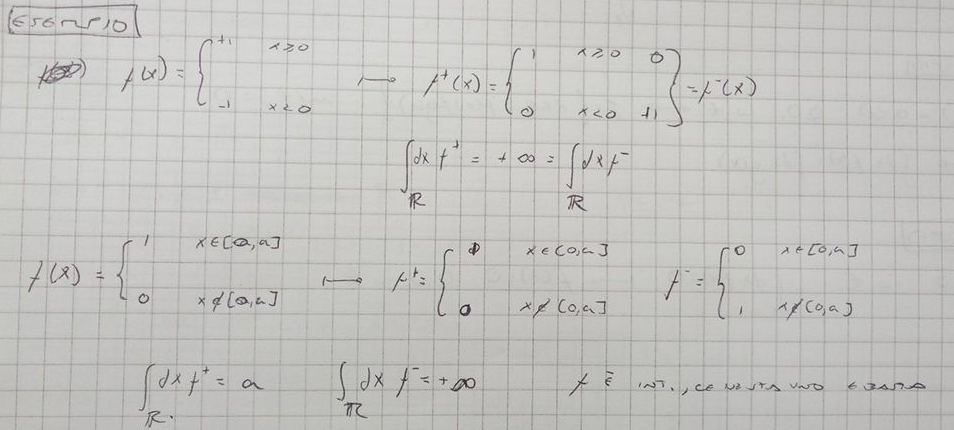
\includegraphics[width=\textwidth]
		{images/fmisintes.png}
		\caption{\label{fig:my-label}}}
\end{figure}


\newpage

\subsection{"Quasi Ovunque"}

Apriamo una brevissima parentesi sul concetto di "Quasi Ovunque", abbreviato \qo (in inglese "Almost Everywhere", A.E.), che ci tornerà utile più avanti.

Si dice che una proprietà è valida \qo in un dominio $A$ se è verificata in tutti i suoi sottoinsiemi tranne quelli a misura nulla.

\begin{figure}[!htb]
	\center{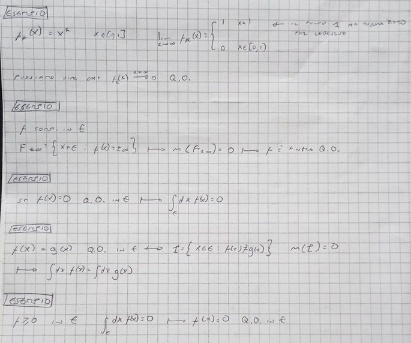
\includegraphics[width=\textwidth]
		{images/qo.png}
		\caption{\label{fig:my-label}}}
\end{figure}

\newpage

\subsection{Criterio del confronto per la sommabilità}

Siano due funzioni
\begin{align}
	f,g \taleche E \subset \R^n \longrightarrow \R
\end{align}

Con $E$ misurabile, e sia che
\begin{enumerate}
	\item $g(\vecx)$ sommabile in $E$, con $g(x)\geq 0$
	\item $f(\vecx)$ misurabile in $E$
\end{enumerate}	

Se $|f(\vecx)|\leq g(x) $ \qo in $E$ allora $f(\vecx)$ è sommabile in $E$.

\subsection{Criterio del confronto asintotico}

Sia $E= [a,b)\subset (-\infty \spacecomma +\infty)$ e siano $f$ e $g$ sommabili in $[a,c]$ con $c<b$ ed esista il limite $\limit{x}{b^-} \frac{f(x)}{g(x)}=l$, avremo allora che
\begin{enumerate}
	\item $l \in (0,+\infty)$
	\begin{align}
		\int_{a}^{b} dx \; f(x) < +\infty \leftrightarrow \int_{a}^{b} dx \; g(x) < +\infty
	\end{align}
	\item $l=0$
	\begin{align}
		\int_{a}^{b} dx \; g(x) < +\infty \implies \int_{a}^{b} dx \; f(x) < +\infty
	\end{align}
	\item $l =+\infty$
	\begin{align}
		\int_{a}^{b} dx \; g(x) = +\infty \implies 	\int_{a}^{b} dx \; f(x) = +\infty
	\end{align}
\end{enumerate}

\begin{figure}[!htb]
	\center{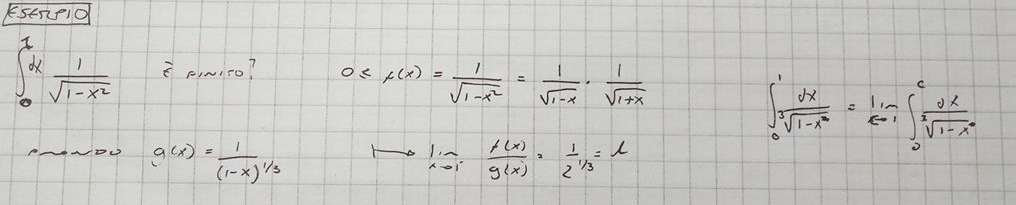
\includegraphics[width=\textwidth]
		{images/confras1.png}
		\caption{\label{fig:my-label}}}
\end{figure}

\begin{figure}[!htb]
	\center{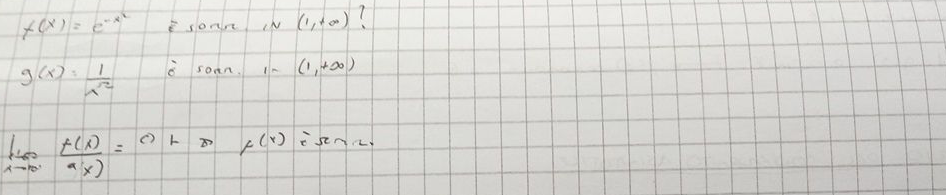
\includegraphics[width=\textwidth]
		{images/confras2.png}
		\caption{\label{fig:my-label}}}
\end{figure}

\subsection{Teorema di passaggio al limite}

Sia la successione di funzioni
\begin{align}
	\{f_n\} \taleche I \subset \R \longrightarrow \R \spacer \{f_n\} \in C^0(I)
\end{align}

Se si ha che $f_n \rightrightarrows f$ in $I$ allora si ha che
\begin{enumerate}
	\item $f\in C^0(I)$
	\item $\int dx \; \limit{n}{\infty}f_n(x)=  \limit{n}{\infty} \int dx \; f_n(x)$ 
\end{enumerate}

Se si ha solo $f_n \longrightarrow f$ il teorema non vale.

\newpage

\subsection{Teorema di convergenza di Poeno-Segre}

Data una successione di funzioni $\{f_n\} \taleche E \subset \R^n \longrightarrow \R$ se vengono rispettate le seguenti condizioni
\begin{enumerate}
	\item $E$ misurabile
	\item $\{f_k(\vecx)\}_{k\geq 1} $
	\item $0\leq f_1(\vecx) \leq f_2(\vecx) \leq \dots \leq f_n(\vecx) $ (la non negatività è opzionale, come vedremo più avanti)
\end{enumerate}

Si avrà che se $f(\vecx)=\limit{k}{\infty}f_k(\vecx)$ allora
\begin{align}
	\limit{k}{\infty} \int_{E} d\vecx \; f_k(\vecx)= \int_{E} d\vecx \; f(\vecx)= \int_{E} d\vecx \;\limit{k}{\infty}  f_k(\vecx)
\end{align}

Perché la non negatività è una condizione opzionale? Perché basta trovare una $g(\vecx)\leq f_1(\vecx)$ e definire
\begin{align}
	F_k(\vecx)= -g(\vecx) + f_k(\vecx)
\end{align}

Che sarà per forza non negativa, e quindi si può applicare il teorema su questa.

\begin{figure}[!htb]
	\center{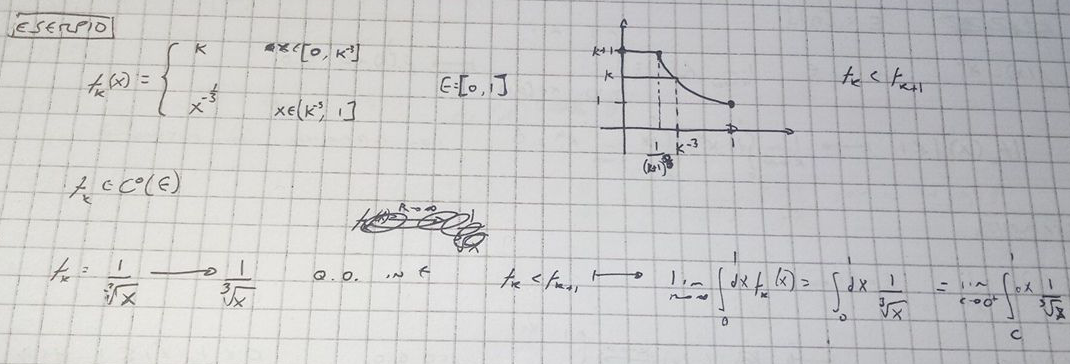
\includegraphics[width=\textwidth]
		{images/conps.png}
		\caption{\label{fig:my-label}}}
\end{figure}

\subsection{Scambio tra somma e integrale per serie a termini non negativi}

Sia una serie
\begin{align}
	\{u_k(\vecx)\}_{k\geq 1} \spacer u_k(\vecx) \geq 0 \quad \forall k \spacecomma \forall \vecx \in E \subset \R^n
\end{align}

E siano $E$ misurabile e gli $u_k$ integrabili in $E$. 

Possiamo definire
\begin{align}
	f_k(\vecx) = \sum_{j=1}^{k} u_j(\vecx) \spacer k \geq 1
\end{align}

Da cui possiamo ricavare
\begin{align}
	f_{k+1} = f_k + u_{k+1} \geq f_k
\end{align}

Il che ci permette di scrivere
\begin{align}
	\limit{k}{\infty} \int_{E} d\vecx \; \sum_{j=1}^{k} u_j(\vecx) = 
	\int_{E} d\vecx \; \limit{k}{\infty}\sum_{j=1}^{k} u_j(\vecx)
\end{align}

Nel termine a sinistra la serie è a termini finiti, e quindi per linearità possiamo invertire serie e integrale e scrivere
\begin{align}
	\limit{k}{\infty}  \sum_{j=1}^{k} \int_{E} d\vecx \; u_j(\vecx) = \sum_{j=1}^{+\infty} \int_{E} d\vecx \; u_j(\vecx) \end{align}

mentre nel secondo termine semplicemente scriviamo
\begin{align}
	\limit{k}{\infty}\sum_{j=1}^{k} u_j(\vecx) = \sum_{j=1}^{+\infty} u_j(\vecx)
\end{align} 

E otteniamo quindi
\begin{align}
	\sum_{j=1}^{+\infty}  \int_{E} d\vecx \;  u_j(\vecx) = \int_{E} d\vecx \; \sum_{j=1}^{+\infty} u_j(\vecx)
\end{align}

\newpage

\subsection{Teorema di Lebesgue per la convergenza dominata}

Se vengono rispettate le seguenti condizioni
\begin{enumerate}
	\item $E\subset \R^n$ misurabile
	\item $\{ f_k(\vecx) \}$ integrabile in $E$ e tale che $\exists f(\vecx)= \limit{k}{\infty} f_k(\vecx)$
	\item $\exists g(\vecx) \geq 0$ sommabile in $E$ tale che $|f_k(\vecx)| \leq g(\vecx)$ \qo in $E$
\end{enumerate}

Allora si ha che
\begin{align}
	\limit{k}{\infty} \int_{E} d\vecx \; f_k(\vecx)= \int_{E} d\vecx \; f(\vecx)= \int_{E} d\vecx \;\limit{k}{\infty}  f_k(\vecx) 
\end{align}

Non dimostriamo il teorema, perché so' conti e non ci serve dimostrarlo.

\bigskip

Rispetto a Poeno-Segre abbiamo l'esistenza di $g(\vecx)$ che domina sia la successione che la funzione a cui tende. Questo ci torna utile qualora ci si trovi a lavorare con una successione limitata. Infatti se $\exists M>0 \taleche |f_k(\vecx)|\leq M$ \qo in $E$ e si ha che $m(E)< + \infty$ possiamo definire
\begin{align}
	g(\vecx)= M \chi_E(\vecx)
\end{align}
E possiamo quindi applicare il teorema di Lebesgue.

\bigskip

Un'altra conseguenza del teorema è che per il teorema del confronto le $f_K(\vecx)$ sono anche sommabili in $E$.

\begin{figure}[!htb]
	\center{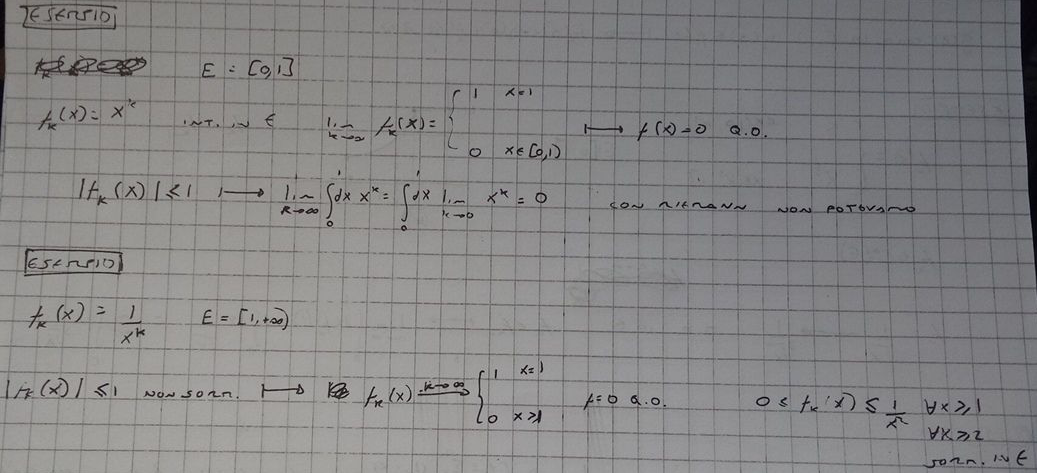
\includegraphics[width=0.9\textwidth]
		{images/convdom.png}
		\caption{\label{fig:my-label}}}
\end{figure}

\newpage


\subsection{Spazi di Lebesgue $L^p$}

Dato un dominio $E\subset \R^n$ misurabile, possiamo definirvi sopra degli spazi $L^p$. Iniziamo col grado più basso, ovvero
\begin{align}
	L^1(E) = \left\{ f \taleche E \subset \R^n \longrightarrow \R \spacecomma \int_{E} d\vecx \; |f(\vecx)|< + \infty  \right\}
\end{align}

$L^1(E)$ è uno spazio normato, con
\begin{align}
	||f||_1 = \int_{E} d\vecx \; |f(\vecx)|
\end{align}

Generalizziamo al caso $L^p$
\begin{align}
	L^p(E) = \left\{ f \taleche E \subset \R^n \longrightarrow \R \spacecomma \int_{E} d\vecx \; |f(\vecx)|^p< + \infty  \right\}
\end{align}

Anche $L^p(E)$ è uno spazio normato, con
\begin{align}
	||f||_p = \left(\int_{E} d\vecx \; |f(\vecx)|^p \right)^{\fracn{p}}
\end{align}

Gli spazi $(L^p \spacecomma ||\cdot||_p)$ sono anche spazi di banach, ovvero normati e completi. 

Inoltre gli elementi dello spazio sono classi di equivalenza rispetto alla relazione $f=g$ \qo in $E$.

\bigskip

Un caso particolarmente interessante si ha per $p=2$, che è anche spazio di Hilbert, dove si ha anche definito il prodotto scalare!
\begin{align}
	||f||_2= \left(\int_{E} d\vecx \; |f(\vecx)|^2 \right)^{\fracn{2}} \spacer \braket{f|g} = \int_{E} d\vecx \; f(\vecx)\cdot g(\vecx)
\end{align}

\subsection{Derivazione sotto segno di integrale}

Prendiamo in considerazione un dominio $E\subset \R^n$ misurabile, un dominio $A=(c,d)\subset \R$ aperto e sia
\begin{align}
	f \taleche E \times A {}& \longrightarrow \R\\
	(\vecx,t) & \longrightarrow f(\vecx,t) \nonumber
\end{align}

Fissiamo $t$ in modo tale che $f(\cdot , t)$ sia integrabile in $A$ e definiamo
\begin{align}
	F(t)= \int_{E} d\vecx \; f(\vecx,t) \spacer t\in A
\end{align}

Ci chiediamo ora. quando è possibile scambiare l'integrale rispetto a $\vecx$ e la derivata rispetto a $t$? 

Innanzitutto dobbiamo assicurarci che $F$ sia continua. Per questo ci viene in aiuto il seguente \textbf{teorema:}

\bigskip

\textit{Se vengono rispettate le seguenti condizioni:}
\begin{enumerate}
	\item $f \taleche \vecx \longrightarrow f(\vecx,t)$ \textit{è sommabile in E $\forall t \in A$}
	\item $f \taleche t \longrightarrow f(\vecx,t)$ \textit{è continua \qo in $A$ $\forall \vecx \in E$}
	\item $\exists g(\vecx)$ \textit{sommabile in $E$ tale che $f(\vecx,t)\leq g(\vecx) \quad \forall t \in A \spacecomma \forall \vecx \in E$ \qo}
\end{enumerate}

\textit{Allora $F(t)$ è continua in $A$.}

\bigskip

Per la dimostrazione, piuttosto che verificare
\begin{align}
	\limit{t}{t_0} F(t) \doubteq F(t_0)
\end{align}

Riscriviamo il problema come
\begin{align}
	\limit{k}{\infty} F(t_k) \doubteq F(t_0) \quad \forall \{ t_k \}_{k\geq 1} \taleche t_k \longrightarrow t_0
\end{align}

Ci troviamo quindi con
\begin{align}
	\limit{k}{\infty} F(t_k) = \limit{k}{\infty} \int_{E} d\vecx \; f(\vecx,t_k)
\end{align}
Grazie alla terza ipotesi possiamo applicare il th. di convergenza dominata, e quindi scrivere
\begin{align}
	\limit{k}{\infty} F(t_k) = \int_{E} d\vecx \; \limit{k}{\infty} f(\vecx,t_k)
\end{align}
Grazie alla seconda ipotesi possiamo scrivere
\begin{align}
	\limit{k}{\infty} f(\vecx,t_k) = f(\vecx,t_0)
\end{align}
E quindi ci troviamo ad avere
\begin{align}
	\limit{k}{\infty} F(t_k) = \int_{E} d\vecx \; f(\vecx,t_0) = F(t_0)
\end{align}
E il teorema è dimostrato.

\bigskip

Ora che ci siamo assicurati di avere fra le mani una funzione continua possiamo enunciare il seguente \textbf{teorema:}

\bigskip

\textit{Se vengono rispettate le seguenti condizioni:}
\begin{enumerate}
	\item $f \taleche \vecx \longrightarrow f(\vecx,t)$ \textit{è sommabile in E $\forall t \in A$}
	\item $f \taleche t \longrightarrow f(\vecx,t)$ \textit{è continua \qo in $A$ $\forall \vecx \in E$}
	\item $\exists g(\vecx)$ \textit{sommabile in $E$ tale che $f(\vecx,t)\leq g(\vecx) \quad \forall t \in A \spacecomma \forall \vecx \in E$ \qo}
	\item $f \taleche t \longrightarrow f(\vecx,t)\in C^1(A) \leftrightarrow f_t(\vecx,t)\in C^0(A)$ 
	\item $\exists g_1(\vecx)$ \textit{sommabile in $E$ tale che $f_t(\vecx,t)\leq g_1(\vecx) \quad \forall t \in A \spacecomma \forall \vecx \in E$ \qo}
\end{enumerate}

\textit{Allora avremo che}
\begin{align}
	F(t)\in C^1(A) \spacer F'(t)= \int_{E} d\vecx \; \partialder{}{t}f(\vecx,t)
\end{align}

\bigskip
Per la dimostrazione procediamo in modo analogo a prima. 

Invece di verificare che
\begin{align}
	\exists \limit{t}{t_0} \frac{F(t) - F(t_0)}{t-t_0} = \text{quantità finita}
\end{align}

Verifichiamo che
\begin{align}
	\exists \limit{k}{\infty} \frac{F(t_k) - F(t_0)}{t_k-t_0} = \text{quantità finita} \quad \forall \{ t_k \}_{k\geq 1} \taleche t_k \longrightarrow t_0
\end{align}

Iniziamo scrivendo il rapporto incrementale
\begin{align}
	\frac{F(t_k) - F(t_0)}{t_k - t_0}
\end{align}

Per linearità possiamo scrivere
\begin{align}
	\frac{F(t_k) - F(t_0)}{t_k - t_0} = \int_{E} d\vecx \; \frac{f(\vecx,t_k) - f(\vecx,t_0)}{t_k - t_0}
\end{align}

Utilizzando il th. di Lagrange avremo
\begin{align}
	\int_{E} d\vecx \; \frac{f(\vecx,t_k) - f(\vecx,t_0)}{t_k - t_0} = \int_{E} d\vecx \; \partialder{}{t}f(\vecx,\xi_k) \spacer \xi_k \in I(t_k,t_0)
\end{align}

Passando a limite, facendo uso del th. della conv. dominata e della continuità della derivata avremo
\begin{align}
	\limit{k}{\infty} \frac{F(t_k) - F(t_0)}{t_k - t_0} {}&= \limit{k}{\infty} \int_{E} d\vecx \; \partialder{}{t}f(\vecx,\xi_k) = \continue
	&= \int_{E} d\vecx \; \limit{k}{\infty} \partialder{}{t}f(\vecx,\xi_k) =  \quad \text{[conv. dominata]}\continue
	&= \int_{E} d\vecx \;  \partialder{}{t}f(\vecx,t_0)  \quad \text{[continuità della der.]}
\end{align}

E il teorema è così dimostrato.

\begin{figure}[!htb]
	\center{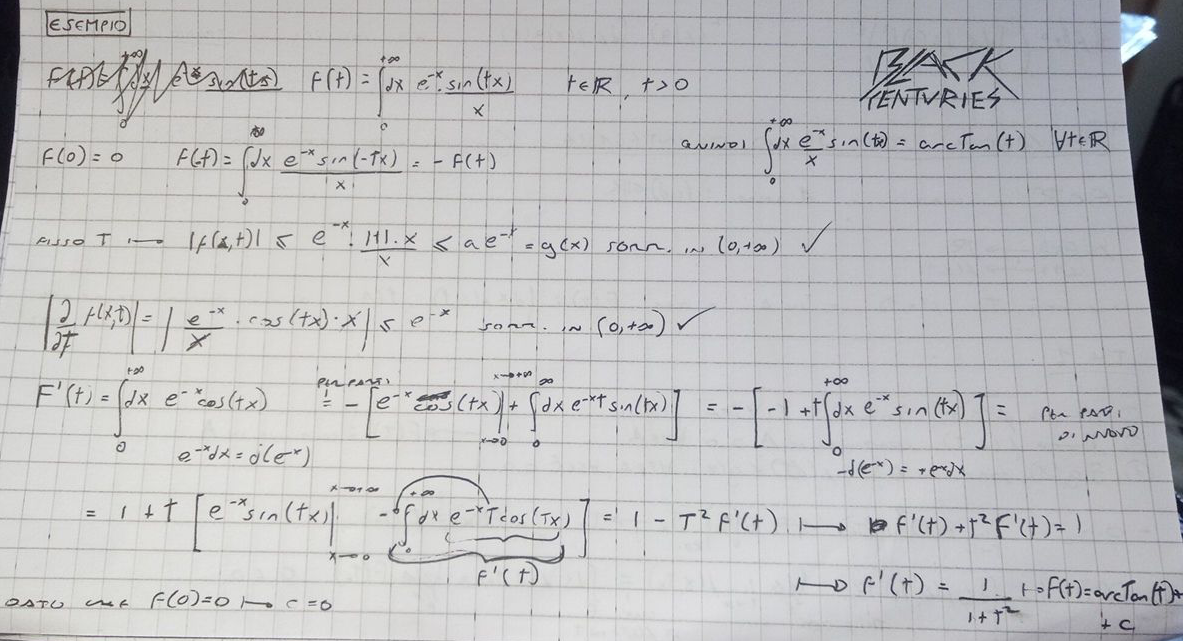
\includegraphics[width=\textwidth]
		{images/derint.png}
		\caption{\label{fig:my-label}}}
\end{figure}
\newpage

FOGLIO 25 BLOCKNOTES NON SI CAPISCE UN CAZZO

\newpage

\subsection{Misura di insiemi in $\R^2$}

Per effettuare la misura di un insieme $E$ in $\R^2$ come quello in figura si può procedere in due modi:

\begin{figure}[!htb]
	\center{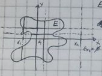
\includegraphics[width=0.3\textwidth]
		{images/misins.png}
		\caption{\label{fig:my-label}}}
\end{figure}

\begin{enumerate}
	\item \textbf{Fissando la $x$}
	\begin{align}
		E_x = \{y \in \R \taleche (x,y)\in E \} \spacer 		m_2(E)= \int_{R}dx \; m_1(E_x) 
	\end{align}
	\item \textbf{Fissando la $y$}
	\begin{align}
		E_y = \{y \in \R \taleche (x,y)\in E \} \spacer m_2(E)= \int_{R}dy \; m_1(E_y) 
	\end{align}
\end{enumerate}

Un insieme si dice
\begin{enumerate}
	\item \textbf{Normale rispetto all'asse $x$} se si ha che
	\begin{align}
		{}&E= \{ (x,y)\in \R^2 \taleche x\in[a,b] \spacecomma y \in [\alpha(x) \spacecomma \beta(x)]   \}\\
		&\alpha(x) \spacecomma \beta(x) \in C^0([a,b]) \spacer \alpha(x) \leq \beta(x) \quad \forall x \in [a,b]
	\end{align}
	\begin{figure}[!htb]
		\center{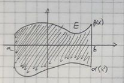
\includegraphics[width=0.3\textwidth]
			{images/misins2.png}
			\caption{\label{fig:my-label}}}
	\end{figure}
	
	In questo caso
	
	\begin{align}
		{}&E_x = \double{\emptyset \quad {}& x \notin [a,b]}{\{  y\in \R \taleche y \in [\alpha(x) \spacecomma \beta(x)]  \} \quad & x \in [a,b]} \\
		& m_1(E_x) = \beta(x) - \alpha(x) \implies m_2(E) = \int_{a}^{b} dx \; [\beta(x) - \alpha(x)]
	\end{align}
	
	
	
	\item \textbf{Normale rispetto all'asse $y$} se si ha che
	\begin{align}
		{}&E= \{ (x,y)\in \R^2 \taleche y\in[c,d] \spacecomma x \in [\gamma(y) \spacecomma \delta(x)]   \}\\
		&\gamma(y) \spacecomma \delta(y) \in C^0([c,d]) \spacer \gamma(y) \leq \delta(y) \quad \forall y \in [c,d]
	\end{align}
	\begin{figure}[!htb]
		\center{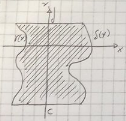
\includegraphics[width=0.3\textwidth]
			{images/misins3.png}
			\caption{\label{fig:my-label}}}
	\end{figure}
	In questo caso
	
	\begin{align}
		{}&E_y = \double{\emptyset \quad {}& y \notin [c,d]}{\{  x\in \R \taleche x \in [\gamma(y) \spacecomma \delta(y)]  \} \quad & y \in [c,d]} \\
		& m_1(E_y) = \delta(y) - \gamma(y) \implies m_2(E) = \int_{c}^{d} dy \; [\delta(y) - \gamma(y)]
	\end{align}
\end{enumerate}

Ovviamente non è detto che se un insieme è normale rispetto ad un asse lo sarà anche rispetto all'altro.

\newpage

ESEMPI SU FOTO SCOMODI DA FOTOGRAFARE, COPIARE POI

\newpage


\subsection{Teorema di Fubini}

Supponiamo di avere una $f(x,y)$ sommabile in $\R^2$. Allora se si ha che
\begin{enumerate}
	\item Fissato $x$ e considerata $f(y)$, essa è sommabile in $\R$.
	
	$f(y) \taleche y \longrightarrow f(x,y)$ è sommabile in $\R$ per $x$ fissato \qo se è ben definito $\int_{R} dy \; f(x,y) = g(x)$  
	
	\item $g(x)$ è sommabile in $\R$ 
\end{enumerate}

Allora si avrà che
\begin{align}
	\iint_{\R^2}dxdy \; f(x,y) = \int_\R dx \; \int_\R dy \; f(x,y)
\end{align}

Oppure, invertendo le variabili nelle ipotesi si avrà
\begin{align}
	\iint_{\R^2}dxdy \; f(x,y) = \int_\R dy \; \int_\R dx \; f(x,y)
\end{align}

\bigskip

Ma c'è un problema! Per come lo abbiamo definito, il teorema non considera domini finiti. E quindi, data una funzione continua definita su $E = \{ (x,y)\in \R^2 \taleche x\in[a,b] \spacecomma y \in [\alpha(x), \beta(x)] \}$, come calcoliamo l'integrale sul dominio? Basta farci furbi e definire
\begin{align}
	f^*(x) = f(x) \cdot \chi_E(x) = \double{f(x) \quad {}& (x,y)\in E }{0 \quad & (x,y) \notin E}
\end{align}

E applicare il th. di Fubini su questa funzione.  Questo ci permette di scrivere
\begin{align}
	{}&\iint_{\R^2}dxdy \; f^*(x,y) = \int_\R dx \; \int_\R dy \; f^*(x,y)\nextpassage
	&\iint_{E}dxdy \; f(x,y) = \int_{a}^{b} dx \; \int_{\alpha(x)}^{\beta(x)} dy \; f(x,y)
\end{align}

\newpage

ESEMPI CHE NON POSSO SCANNARE, DA TRASCRIVERE POI 

\newpage

\subsection{Centro di Massa di una superficie}

Diamo, in modo analogo al caso di una curva, la definizione di baricentro (o CDM) di una superficie $E$ con densità $\rho(x,y)>0$
\begin{align}
	x_B = \frac{\iint_E dxdy \; x\cdot \rho(x,y)}{\iint_E dxdy \;  \rho(x,y)} \spacer y_B = \frac{\iint_E dxdy \; y\cdot \rho(x,y)}{\iint_E dxdy \;  \rho(x,y)}
\end{align}

\begin{figure}[!htb]
	\center{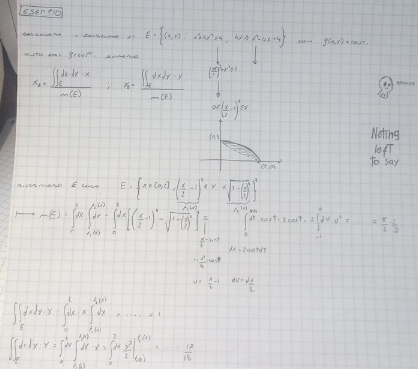
\includegraphics[width=\textwidth]
		{images/cdmsup.png}
		\caption{\label{fig:my-label}}}
\end{figure}

\newpage

\subsection{Calcolo dei volumi}
Dato un insieme $E\subset \R^3$, come troviamo il suo volume?

Fissiamo $z$ in modo tale da avere
\begin{align}
	E_z= \{(x,y) \taleche (x,y,z) \in E\}\subset \R^2
\end{align}

Possiamo procedere come per il caso in $\R^2$, "affettando" il dominio $E$ perpendicolarmente a $z$, e calcolando $m_2(E_z)$, per infine ottenere
\begin{align}
	m_3(E)= \int_{R} dz \; m_2(E_z)
\end{align}

Questo metodo viene chiamato \textbf{Integrazione per strati}.

\begin{figure}[!htb]
	\center{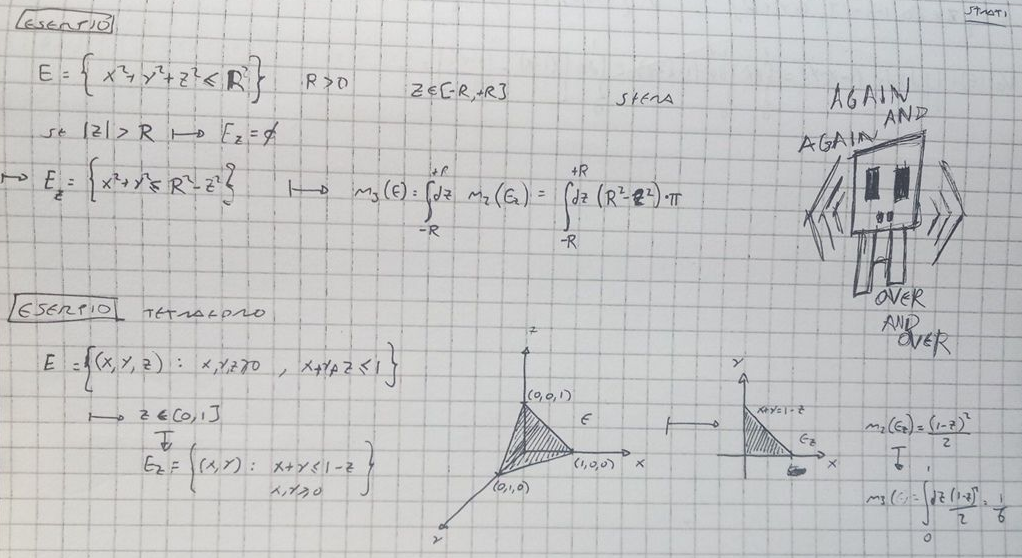
\includegraphics[width=0.6\textwidth]
		{images/intstr.png}
		\caption{\label{fig:my-label}}}
\end{figure}

Alternativamente si può procedere \textbf{per fili}, ovvero dividendo il dominio $E$ nel seguente modo
\begin{align}
	E_{xy} = \{ z \in (x,y,z)\in E \}\subset \R  
\end{align}

Per poi calcolare
\begin{align}
	m_3(E)= \iint_{\R^2} dxdy \; m_1(E_{xy})
\end{align}

\begin{figure}[!htb]
	\center{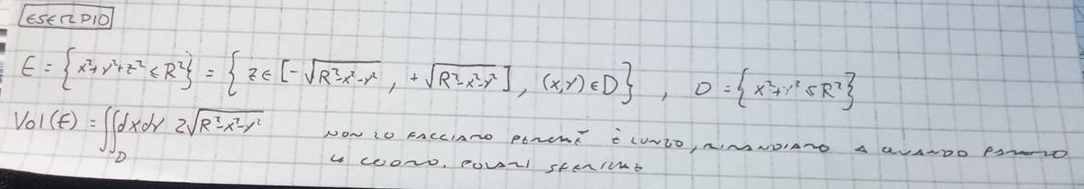
\includegraphics[width=0.7\textwidth]
		{images/intfili.png}
		\caption{\label{fig:my-label}}}
\end{figure}

\subsection{Cambio di variabili (MANCANTE)}

Iniziamo ricordando cos'è un diffeomorfismo. Data
\begin{align}
	g \taleche A \subset \R^n \longrightarrow B \subset \R^n
\end{align}

Con $A$,$B$ aperti. $g$ è un diffeomorfismo se
\begin{enumerate}
	\item $g$ è iniettiva in $A$
	\item															
\end{enumerate}

\newpage

\section{Integrali impropri di Riemann}

Torniamo un attimo agli integrali di Riemann. Gli integrali di Riemann hanno una limitazione: non possono lavorare con intervalli aperti o infiniti. Come si può risolvere questo problema? Utilizzando i limiti.

\subsection{Integrali impropri di Io tipo}

Sia una $f \taleche [a,b) \longrightarrow \R$

Se si ha che
\begin{enumerate}
	\item $f(x)$ è \Rint in $[a,c]$ con $c<b$
	\item Esiste finito $\limit{c}{b^-} \int_{a}^{c} dx \; f(x)$ 
\end{enumerate}

Allora si dice che $f(x)$ è integrabile in senso improprio in $[a,b)$ e si ha che
\begin{align}
	\int_{a}^{b} dx \; f(x)=\limit{c}{b^-} \int_{a}^{c} dx \; f(x)
\end{align}

\begin{figure}[!htb]
	\center{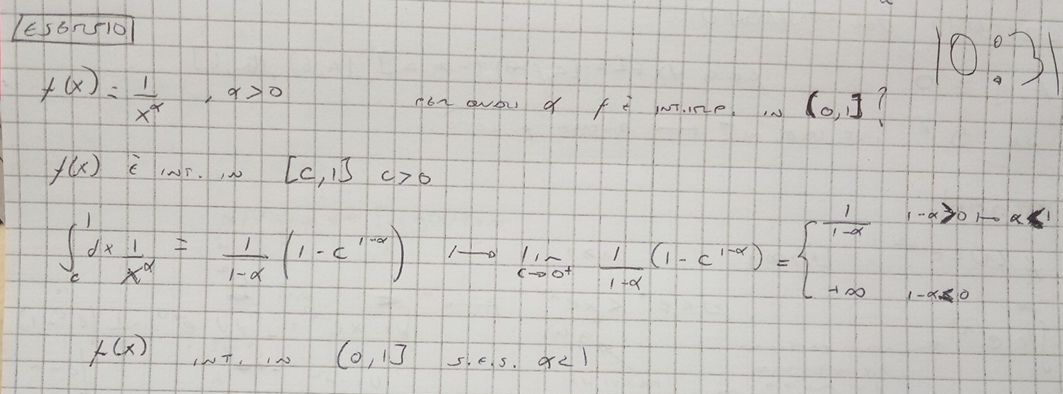
\includegraphics[width=\textwidth]
		{images/intimp1.png}
		\caption{\label{fig:my-label}}}
\end{figure}

\subsection{Integrali impropri di IIo tipo}

Sia ora una $f \taleche [a,+\infty) \longrightarrow \R$

Se si ha che
\begin{enumerate}
	\item $f(x)$ è \Rint in $[a,c]$ con $c>a$
	\item Esiste finito $\limit{c}{\infty} \int_{a}^{c} dx \; f(x)$ 
\end{enumerate}

Allora si dice che $f(x)$ è integrabile in senso improprio in $[a,+\infty)$ 

\begin{figure}[!htb]
	\center{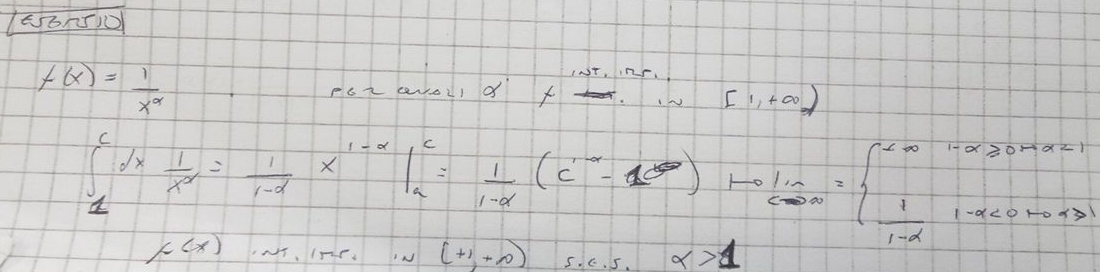
\includegraphics[width=\textwidth]
		{images/intimp2.png}
		\caption{\label{fig:my-label}}}
\end{figure}
\begin{figure}[!htb]
	\center{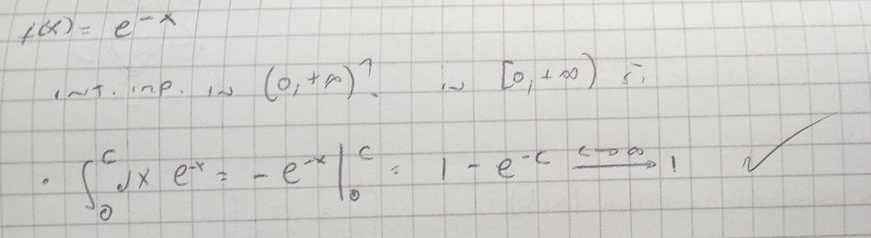
\includegraphics[width=\textwidth]
		{images/intimp3.png}
		\caption{\label{fig:my-label}}}
\end{figure}

\newpage

\subsection{Criterio del confronto per integrali jmpropri}

Siano due funzioni $f,g\geq 0 \taleche f \leq g \quad \forall x \in I=[a, + \infty), (-\infty, +a],[a,b) , (a,b]$  

Se $g$ è integrabile in senso improprio in $I$ allora anche $f$ lo è.

\begin{figure}[!htb]
	\center{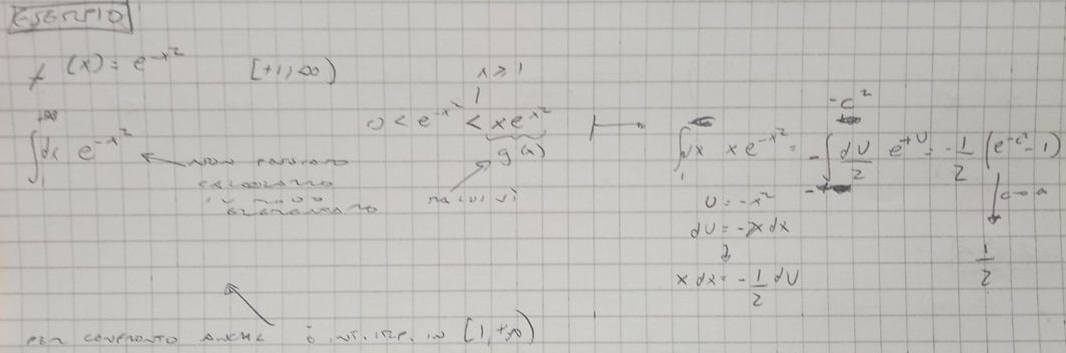
\includegraphics[width=\textwidth]
		{images/intimp4.png}
		\caption{\label{fig:my-label}}}
\end{figure}
